\documentclass{beamer}
\usepackage{geometry}
\usepackage[english]{babel}
\usepackage[utf8]{inputenc}
\usepackage{amsmath}
\usepackage{amsfonts}
\usepackage{amssymb}
\usepackage{tikz}
\usepackage{graphicx}
\usepackage{venndiagram}

%\usepackage{pgfplots}
%\pgfplotsset{width=10cm,compat=1.9}
%\usepackage{pgfplotstable}

\setlength{\headheight}{26pt}%doesn't seem to fix warning

\usepackage{fancyhdr}
\pagestyle{fancy}
\fancyhf{}

%\rhead{\small{5 September 2018}}
\lhead{\small{BECA / Dr. Huson / 11.1 IB Math Unit 1}}

%\vspace{1cm}

\renewcommand{\headrulewidth}{0pt}


\title{Mathematics Class Slides}
\subtitle{Bronx Early College Academy}
\author{Chris Huson}
\date{24 September - 5 October 2018}

\begin{document}

\frame{\titlepage}

\section[Outline]{}
\frame{\tableofcontents}

\section{2.1 Drui: Composite functions} %Monday Sept 24
  \frame
  {
    \frametitle{GQ: How do we combine functions?}
    \framesubtitle{CCSS: HSF.IF.C.7 Analyze functions  \hspace{\stretch{1}}  \alert{2.1}}

    \begin{block}{Do Now: Textbook exercises 1E \# 3-5 pp. 13-14}
    \begin{enumerate}
        \item Write practice problems on loose leaf paper
        \item In your notebook, write the Guiding Question and the date
        \item Take out homework, calculator
    \end{enumerate}
    \end{block}
    Lesson: Function composition, operations p 14-15 \\*[5pt]
    Homework: Problem set: Function operations
  }
%Prepare copies of formula sheets

\section{2.2 Drui: Laptop work with Desmos and Word. Tuesday Sept 25}
  \frame
  {
    \frametitle{How do we communicate mathematical results?}
    \framesubtitle{CCSS: MP.4 Model with mathematics \hspace{\stretch{1}} \alert{2.2}}

    \begin{block}{Technical skills needed to communicate mathematics}
    \begin{enumerate}
        \item Word processing: Microsoft Word and equation editor
        \item Computer calculators: Desmos; domain restriction, labeling
        \item Cloud storage: Dropbox
        \item Technical writing standards: MLA format (Purdue OWL)
        \item Writing style: declarative
        \item Assessment criteria: IB exploration criterion \emph{B: Mathematics Presentation}
    \end{enumerate}
    \end{block}
    Lesson: Shared folder structure, graph copy/paste, MLA template\\ \bigskip
    Homework: Pre-test
  }

\section{2.3 Drui: Inverse functions, Wednesday Sept 26}
  \frame
  {
    \frametitle{GQ: How do we find the inverse of functions?}
    \framesubtitle{CCSS: HSF.IF.C.7 Analyze functions  \hspace{\stretch{1}}  \alert{2.3}}

    \begin{block}{Do Now: Function composition, operations.}
    \begin{enumerate}
        \item Given $f(x)=x-5$ and $g(x)=x^2$. Find $f+g$, $f \circ g$, and $(g \circ f)(3)$
        \item If $r(x)=x-3$ and $s(x)=x^2$, find $(r \circ s)(x)$ and state its domain and range.
    \end{enumerate}
    \end{block}
    Lesson: Function inverses p 16-19; Exercise 1G p.18-19 \\*[5pt]
    Homework: Problem set: Function inverses
  }

\section{2.4 Drui: Inverse functions, Thursday Sept 27}
  \frame
  {
    \frametitle{GQ: How do we find the inverse of functions algebraically?}
    \framesubtitle{CCSS: HSF.IF.C.7 Analyze functions  \hspace{\stretch{1}}  \alert{2.4}}

    \begin{block}{Do Now: Function composition, inverses.}
    \begin{enumerate}
        \item Given $f(x)=2x-1$ and $g(x)=x^2+1$. Find $f+g$, $f \circ g$, and $(g \circ f)(-1)$.
        \item Graph the function $h=\{(-1,0),(1, 2),(3, 1), (4,5)\}$ and its inverse $h^{-1}$.
        \item Sketch $f(x)=e^x$ and its inverse $f^{-1}(x)=\ln x$. (use your calculator table function)
    \end{enumerate}
    \end{block}
    Review formula sheets\\
    Lesson: Function inverses p 19-20; Exercise 1H p.1-8 \\*[5pt]
    Homework: Problem set: Function inverses
  }

\section{2.5 Drui: Transformations, Monday Oct 1}
  \frame
  {
    \frametitle{GQ: How do we transform functions?}
    \framesubtitle{CCSS: HSF.IF.C.7 Analyze functions  \hspace{\stretch{1}}  \alert{2.5}}

    \begin{block}{Do Now: Function composition, inverses.}
    \begin{enumerate}
        \item Given $f(x)=x-2$ and $g(x)=x^2-1$. Find $f \circ g$, and $(g \circ f)(3)$.
        \item Find the inverse of the function $h(x)=5x+2$.
        \item Given a quadratic function with vertex $(3,2)$ and leading coefficient $a=1$. Write down the function in vertex form. Factor the function and state the zeros. Show that in standard form the function is $y=x^2-6x+11$.
    \end{enumerate}
    \end{block}
    Review formula sheets\\
    Lesson: Function inverses p 21-24; Exercise 1I p.1-7 \\*[5pt]
    Homework: Problem set: Function inverses
  }

\section{2.6 Drui: Laptop work with Desmos and Word. Tuesday Oct 2}
  \frame
  {
    \frametitle{How do we communicate mathematical results?}
    \framesubtitle{CCSS: MP.4 Model with mathematics \hspace{\stretch{1}} \alert{2.6}}

    \begin{block}{Technical skills needed to communicate mathematics}
    \begin{enumerate}
        \item Word processing: Microsoft Word and equation editor
        \item Computer calculators: Desmos; domain restriction, labeling
        \item Cloud storage: Dropbox
        \item Technical writing standards: MLA format (Purdue OWL)
        \item Writing style: declarative
        \item Assessment criteria: IB exploration criterion \emph{B: Mathematics Presentation}
    \end{enumerate}
    \end{block}
    Lesson: Shared folder structure, graph copy/paste, MLA template\\ \bigskip
    Homework: Function transformations practice
  }

\section{2.7 Drui: Review, Wednesday Oct 3}
  \frame
  {
    \frametitle{GQ: How do we transform functions?}
    \framesubtitle{CCSS: HSF.IF.C.7 Analyze functions  \hspace{\stretch{1}}  \alert{2.7}}

    \begin{block}{Do Now: Review handout, function composition, inverses.}
    \end{block}
    Scope p.1-29 \\*[5pt]
    Example exam problems\\ \bigskip
    Homework: Study for exam
    }

\section{2.8 Drui: Test, Thursday Oct 4}
  \frame
  {
    \frametitle{GQ: How do we transform functions?}
    \framesubtitle{CCSS: HSF.IF.C.7 Analyze functions  \hspace{\stretch{1}}  \alert{2.8}}

    \begin{block}{Exam: function composition, inverses.}
    \end{block}
    Scope p.1-29 \\ \bigskip
    Homework: Handout review problems
    }

\section{2.9 Drui: Laptop, Deltamath, Desmos /Word. Tuesday Oct 9}
  \frame
  {
    \frametitle{How do we communicate mathematical results?}
    \framesubtitle{CCSS: MP.4 Model with mathematics \hspace{\stretch{1}} \alert{2.9}}

    \begin{block}{Technical skills needed to communicate mathematics}
    \begin{enumerate}
        \item Word processing: Microsoft Word and equation editor
        \item Computer calculators: Desmos; domain restriction, labeling
        \item Cloud storage: Dropbox
        \item Technical writing standards: MLA format (Purdue OWL)
        \item Writing style: declarative
        \item Assessment criteria: IB exploration criterion \emph{B: Mathematics Presentation}
    \end{enumerate}
    \end{block}
    Lesson: Shared folder structure, graph copy/paste, MLA template\\ \bigskip
    Homework: Deltamath followup. Open textbook online
  }

\section{2.10 Drui: Transformations, Monday Oct 10}
  \frame
  {
    \frametitle{GQ: How do we transform functions?}
    \framesubtitle{CCSS: HSF.IF.C.7 Analyze functions  \hspace{\stretch{1}}  \alert{2.10}}

    \begin{block}{Do Now: Asymptotic behavior}
    \begin{enumerate}
        \item Write down the equation of a horizonal line through $(3,2)$
        \item Write down the equation of the axis of symmetry of a parabola having the vertex $(h,k)$
        \item Write down the domain and range of the given parabolic function
        \item Sketch the function $\displaystyle f(x)=\frac{2x-7}{x+1}$, including the asymptotes.
        \item Explain the algebraic features of $f$ leading to the asymptotes
    \end{enumerate}
    \end{block}
    %Review formula sheets\\
    Lesson: Function transformations p 21-24; Exercise 1I p.1-7 \\*[5pt]
    Homework: Complete exercises 1I
  }

\end{document}


\section{1.3 Drui}
  \frame
  {
    \frametitle{GQ: What is asymptotic behavior?}
    \framesubtitle{CCSS: HSF.IF.B.4 Interpret key features of functions and their graphs \hspace{\stretch{1}} \alert{1.3}}

    \begin{block}{Do Now: Graphing functions}
    \begin{enumerate}
        \item Graph \#3a, p. 12 and one other from problem 3. Use 1 cm = 1 unit
    \end{enumerate}
    \end{block}
    Review Average rate of change problem set\\ \bigskip
    Lesson: Rational functions, factoring denominators, asymptotes pp. 8-11
    \\%*[5pt]
    Homework: Function substitution, domain and range
  }

\frame
{
  \frametitle{Domain and range of a function \hspace{\stretch{1}} \alert{1.3}}
  %\framesubtitle{CCSS: HSF.IF.B.4 Interpret key features of functions and their graphs \hspace{\stretch{1}} \alert{1.3}}
  \begin{enumerate}
    \item Write down the domain and range of the function graphed\\*
    \begin{figure}[!ht]
        \centering
        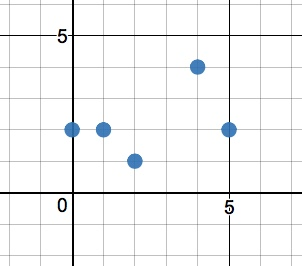
\includegraphics[width=0.35\textwidth]{discrete-domain-graph.jpeg}
    \end{figure}

    \item What is the range of this function modeling a bicycle wheel?
    \begin{figure}[!ht]
        \centering
        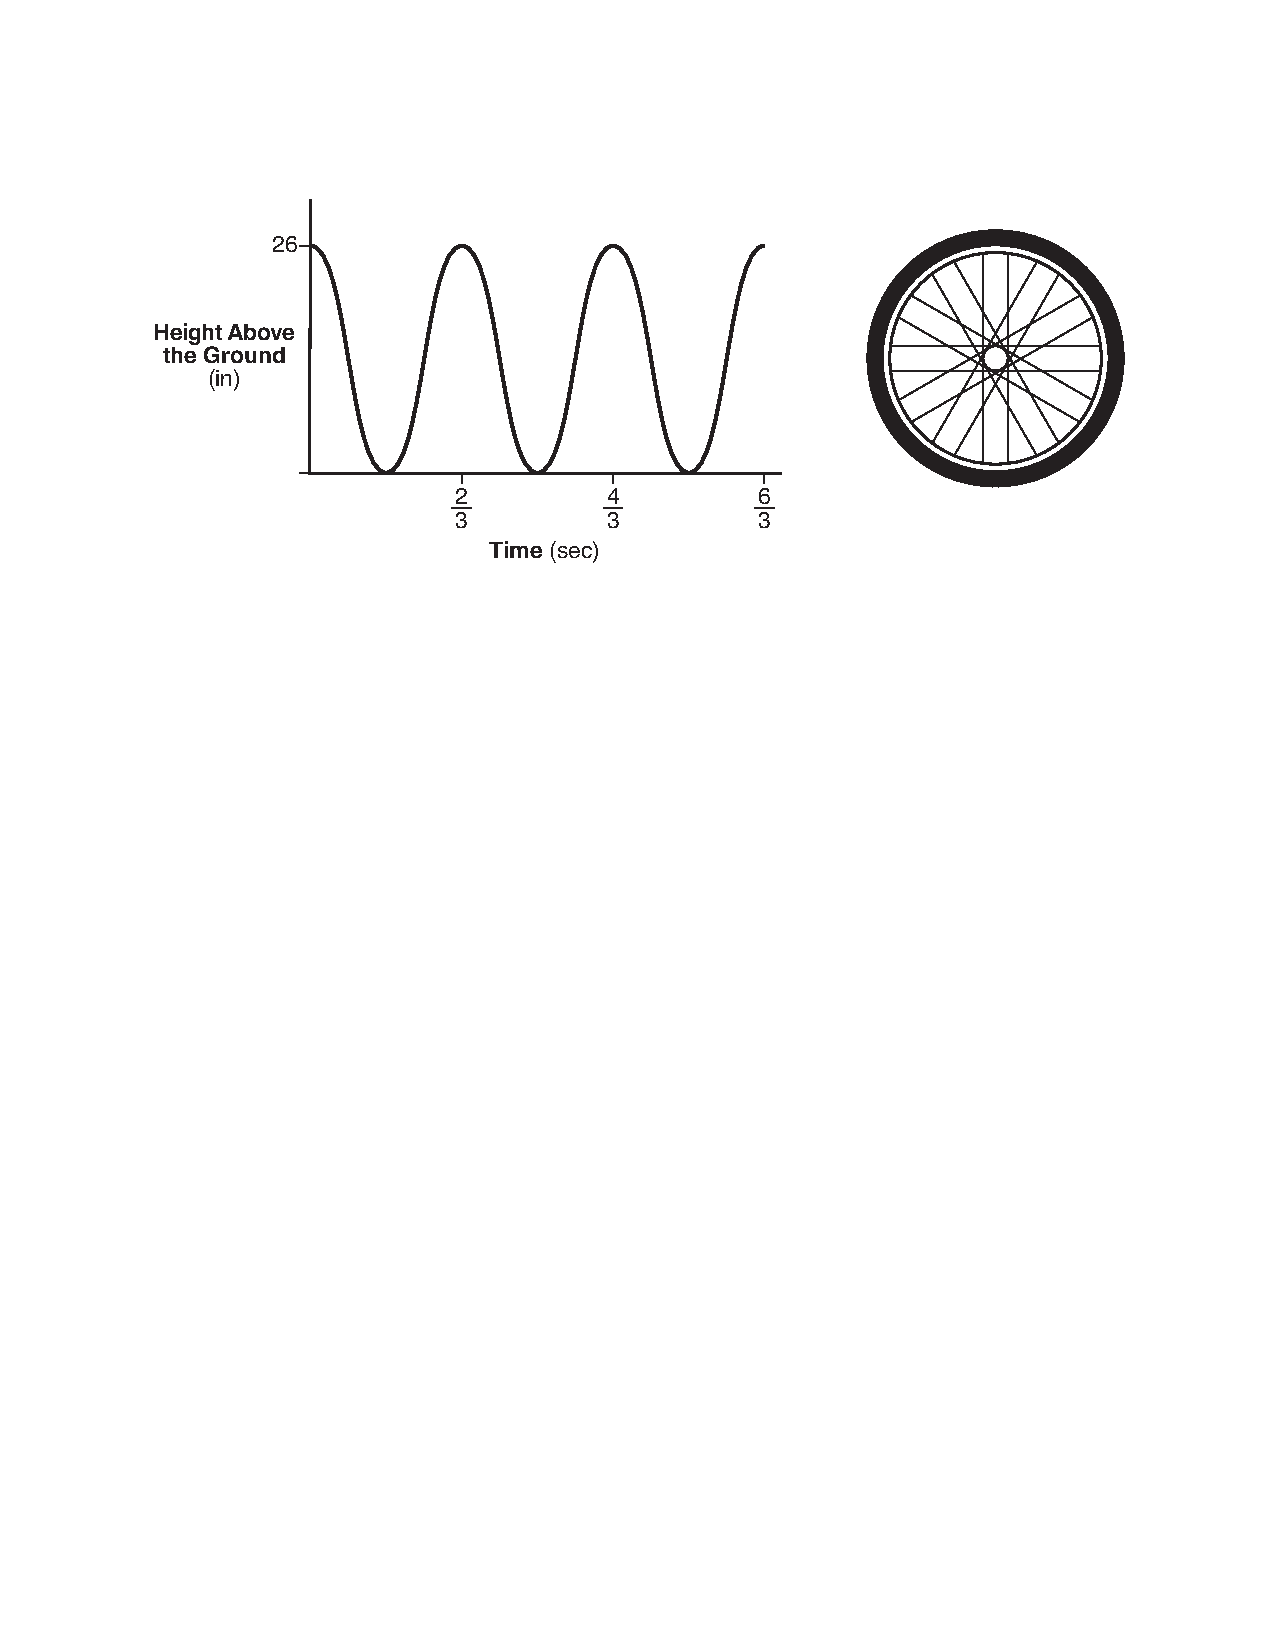
\includegraphics[width=0.70\textwidth]{sine-bike-wheel.pdf}
    \end{figure}
  \end{enumerate}
  }

\frame
{
  \frametitle{Function substitution \hspace{\stretch{1}} \alert{1.3}}
  Given $f(x)=3x+2$. What is $f(2x-1)$? \bigskip
    \begin{enumerate}
        \item Perform the substitution, putting $2x-1$ in parenthesis.\\*[20pt]
        \item Simplify, beginning each line with a leading equals sign if it is equal to the line above.\\*[40pt]
  \end{enumerate}
  }

  \section{1.4 Drui}
  \frame
  {
    \frametitle{GQ: How do we solve quadratic equations?}
    \framesubtitle{CCSS: HSF.IF.B.4 Interpret key features of functions and their graphs \hspace{\stretch{1}} \alert{1.4}}

    \begin{block}{Do Now: Factoring}
    \begin{enumerate}
      \item Find the intercepts, axis of symmetry, and minimum point of the graph of the function $f(x)=(x-1)(x-5)$?
      \item Factor the function $g(x)=x^2-x-12$ to determine the features of its graph.
      \item Convert the function $h(x)=x^2+4x+3$ to the vertex form, $h(x)=a(x-h)^2+k$. Write down its vertex.
    \end{enumerate}
    \end{block}
    Lesson: Factoring, setting $=0$, checking solutions, $x-$ and $y-$intercepts, vertex, axis of symmetry
    \\ \bigskip
    Homework: Factoring practice, completing the square, graphing\\
    Skip around and do what you can by tomorrow
  }

  \section{1.5 Drui - Monday September 17}

  \frame
  {
    \frametitle{How do we graph quadratics?}
    \framesubtitle{CCSS: HSF.IF.B.4 Interpret key features of functions and their graphs \hspace{\stretch{1}} \alert{1.5}}

    \begin{block}{Consider the function $f(x)=-x^2+2x+3$}
    \begin{enumerate}
        \item Factor $f$ and state its zeros.
        \item Restate $f$ in vertex form. Write down the vertex as an ordered pair.
        \item Over what intervals is the function increasing, decreasing, and neither?
        \item If $f(x)$ represents the height of a diver over the domain $0 \leq x \leq 3$, interpret $f(0)$, the vertex, and $f(3)$
        \item What does the "slope" of the curve represent?
    \end{enumerate}
    Lesson: Example 18 p. 54
    \end{block}
  }


\section{1.7 Drui Review Thursday September 20th}
  \frame
  {
    \frametitle{GQ: How do we simplify exponents?}
    \framesubtitle{CCSS: HSN.RN.A.2 Rewrite expressions involving radicals and rational exponents using the properties of exponents \hspace{\stretch{1}} \alert{1.7}}

    \begin{block}{Do Now: Exponent and radicals practice}
      \begin{enumerate}
      \item Exponent product, quotient, and power rules
      \item Fractional exponents
      \item Negative exponents
      \item Graphing exponential function
      \end{enumerate}
   \end{block}
    Lesson: Product, quotient, power rules, $\sqrt{x^4}$ \\ \bigskip
    Homework: Exponent and radicals practice
  }

\section{1.8 Unit exam September 24th}
  \frame
  {
    \frametitle{GQ: How do we use functions in algebra?}
    \framesubtitle{CCSS: HSF.IF.B.4 Interpret key features of functions and their graphs \hspace{\stretch{1}} \alert{1.8}}

  Exam \\ \bigskip
  Homework: Pre-test
  }
